%%----------Chapter 2------------------------------------------
\chapter{How  It Works}\label{chap:background}
Measuring the movement of bodies in three dimensional space is not a new field of study.
Especially in our current age of electronics, one can simply grab an accelerometer and microcontroller off of Amazon, have it delivered in 48 hours, and know the experiences felt by a racetrack car or be able to orient a 3D rendering of a bunny \footnote[1]{https://learn.adafruit.com/adafruit-bno055-absolute-orientation-sensor/overview}.
What makes today exciting is that improvements in manufacturing and computational density have drastically increased the capabilities of small embedded systems.
Now, every cell phone has a sophisticated suite of sensors built into them and they have the simple task of detecting whether the phone is in a landscape or portrait mode. 
Some applications, like Google Maps, have gone further and fused the sensor data, along with GPS information, into a robust navigation system.

\section{Sensing} \label{sec:bkg_imu}
Sensing motion within a 3D environment is a key part of any body tracking problem.
How can we compute the position, velocity, acceleration, and attitude of a body in space?
In order to answer this question, we must first examine the different sensors that are available.

\subsection{Accelerometer} \label{ssec:bkg_accelerometer}
Accelerometers measure a change in velocity over time (acceleration).
An accelerometer is comprised of a mass suspended in an axis of motion by springs of a known K-constant [CITE - Robotics, Vision and Control].
The displacement of the mass along the axis, imparted by a force, is correlated to a sensitivity scale.
Typically, this scale is electrically resistive and creates an analog change in a driving (exciting) voltage.
A basic representation of a three-axis accelerometer is shown in Figure \ref{fig:accelerometers}.

\begin{figure}[h!]
    \caption[Accelerometer block diagram]{Basic block diagram of a three-axis accelerometer where the masses are suspended from springs.}
    \label{fig:accelerometers}
    \centering
    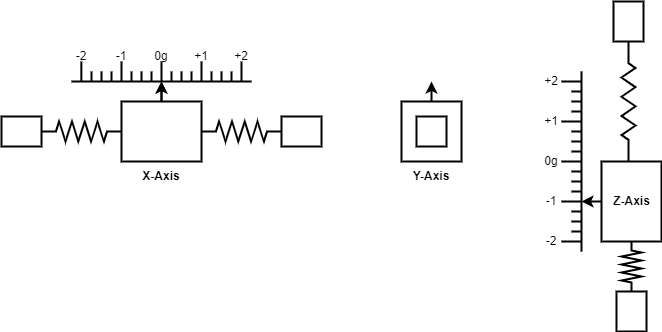
\includegraphics[width=4.5in]{background/accelerometers.png}
\end{figure}

\subsection{Gyroscope} \label{ssec:bkg_gyroscope}
A gyroscope is an inertial sensor that measures the angular velocity of a rotating body.
MEMS-based gyroscopes measure this value by applying the Coriolis effect on a microscopic mass [CITE - Robotics, Vision and Control].

\begin{figure}[h!]
    \caption[Gyroscope block diagram]{Basic block diagram of a three-axis gyroscope where the masses are suspended from springs. The left diagram shows a single mass configuration; the right shows a tuning fork configuration which is twice as sensitive as the singular mass.}
    \label{fig:gyroscopes}
    \centering
    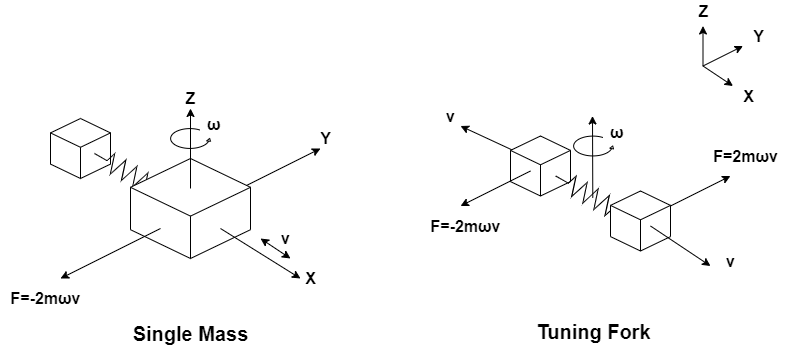
\includegraphics[width=4.5in]{background/gyroscopes.png}
\end{figure}

As shown in Figure \ref{fig:gyroscopes}, an oscillation is induced on the x-axis using a driving circuit.
While oscillating, if an angular velocity ($\omega$) is imparted on the z-axis, the suspended mass will experience a force in the y-axis that is proportional to $\omega$.
The proof for this relationship can be found in Appendix [INSERT APPENDIX NUMBER].

\subsection{Magnetometer} \label{ssec:bkg_magnetometer}
Magnetometers use magnetoresistive elements that change their effective resistance in the presence of a magnetic field [CITE - Robotics, Vision and Control].
Atoms within a magnetoresistive element change their orientations with the magnetic field.
The new orientation can hinder or aid the path of free electrons moving through the element, thus changing the resistance.
By measuring this value and correlating it to a measurement scale, the local magnetic field can be determined.

\begin{figure}[h!]
    \caption[Magnetometer block diagram]{Basic block diagram of a single-axis magnetometer where electrons are flowing through the magnetoresistive material. The left diagram shows the condition when the magnetic field is aligned (minimal resistance); the right shows the non-aligned magnetic field condition which increases the resistance the electrons face passing through the material.}
    \label{fig:magnetometer}
    \centering
    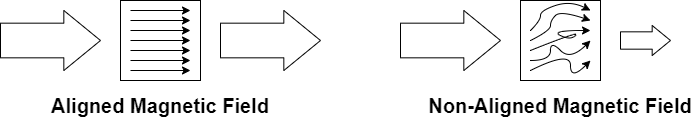
\includegraphics[width=4.5in]{background/magnetometer.png}
\end{figure}

\subsection{Inertial Measurement Units}
Now, with the basics of each inertial sensor in mind, we can combine them into a single package, called an inertial measurement unit (IMU).
Each of the diagrams of the above sensors represent a single sensing axis, or Degree of Freedom (DOF).
In order for our IMU to be useful in a 3D environment, we need to have three sensing axes 90 degrees to each other.
Each DOF will measure the X-, Y-, and Z-axis, respectively with the positive sensing direction according to the right hand rule.
By combining multiple tri-axial arrays, we can define different types of IMUs, as shown in Table \ref{tab:imu_dofs}.
Typically, the more sensing axes, the more accurate the IMU will be (depending on the performance of the sensor fusion algorithm).

\begin{table}[h]
    \caption{Common definitions for IMUs of varying degrees of freedom.}
    \label{tab:imu_dofs}
    \centering
    \begin{tabular}{| c | c | c | c | c |}
        \hline
        DOFs & Accelerometer & Gyroscope & Magnetometer & Barometer \\
        \hline
        3-DOF & 3-axis\footnote[2]{can be either or} & 3-axis\footnote[2] & --- & --- \\
        6-DOF & 3-axis & 3-axis & --- & --- \\
        9-DOF & 3-axis & 3-axis & 3-axis & --- \\
        10-DOF & 3-axis & 3-axis & 3-axis & 1-axis \\
        \hline
    \end{tabular}
\end{table}

\begin{figure}
    \begin{fitbox}[frametitle=Aside: MEMS Technology]
        During the Apollo program, the ST124-M inertial measurement unit was developed that fed the Saturn V rocket's inertial characteristics to the main flight computer [CITE - ST124-M description].
        The IMU consisted of a tri-axial gyroscope array, redundant tri-axial accelerometer arrays, pendulums, and other sensors.
        While it was a technological marvel at the time, it was the size of a basketball and weighed about 45-65 kilograms.
        Modern cellphones with the same capability are orders of magnitude smaller, lighter, and cheaper; so, what happened?

        \begin{center}
            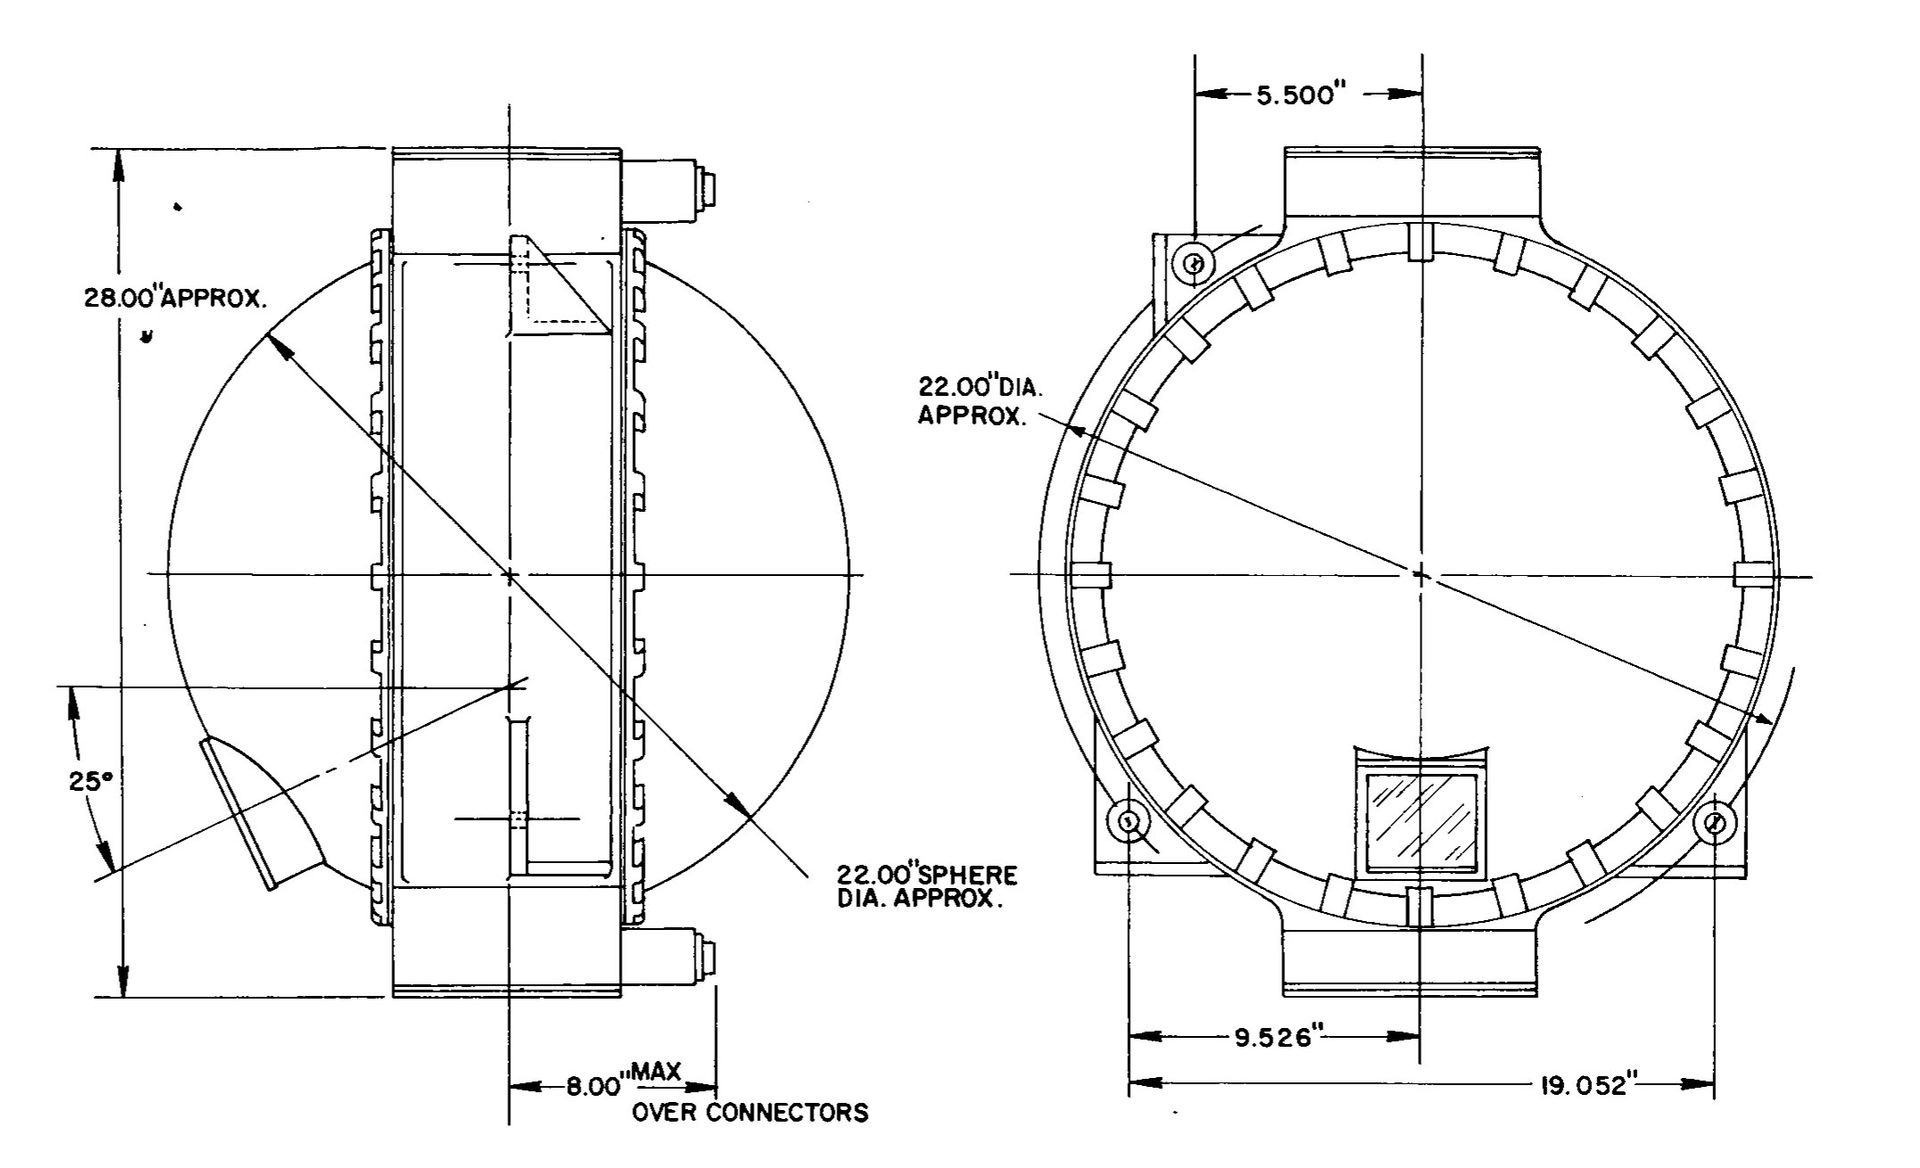
\includegraphics[height=3in]{images/background/Apollo_IMU_exhibit.jpg}
            % \caption[Test]{ST124-M inertial measurement unit courtesy of NASA \url{https://en.wikipedia.org/wiki/ST-124-M3_inertial_platform#/media/File:ST124-M_drawing.jpg}}
            \caption[ST124-M Outline]{ST124-M inertial measurement unit courtesy of NASA via Wikimedia Commons [CITE - Wikimedia]}
        \end{center}

        Modern manufacturing methods have introduced new technology called Microelectromechanical Systems, or MEMS.
        MEMS are microscopic devices that perform an electromechanical function such as sensing acceleration, rotation rate, or magnetic fields [CITE - What is MEMS].
        They are the most common technology in modern sensor development and revolutionized the technology space by shrinking components down to the micro- and nanometer scales.
        Due to the advent of MEMS technology, devices such as accelerometers, magnetometers, gyroscopes, barometers, hygrometers, etc. have been shrunk down from large mechanical masterpieces to mass-producible products that fit within a few square millimeters of epoxy.
        This dramatically cheapened these devices and has allowed more products to integrate smart sensors into their designs.
    \end{fitbox}
\end{figure}

According to VectorNav [CITE], a producer of industrial-grade IMUS, the cheapest, least precise, and least accurate IMUs are considered "consumer-grade".
Every day smartphones, cheap commercial breakout boards, and even shipping crates have these devices on-board.
Consumer-grade IMUs can be bought for cents, dollars, or tens of dollars per unit in bulk and are ideal for mass production spaces where quantity is king over quality.
A step up from these sensors are "industrial-grade" IMUs. 
These are tens to hundreds of dollars per unit but are an order of magnitude more accurate and precise than their consumer counter parts.
This makes them desirable for the automotive and industrial sectors as they can assist in automation, control, and monitoring of expensive unmanned systems.
The "tactical-grade" sensors are even more robust and accurate than the previous tiers and have an appropriate military-industrial complex price tag to match. 
These devices will typically be used in applications where war fighters need precise guidance for munitions, or need to navigate their way through hazardous and GNSS-denied terrain.
Finally, the last major tier is the "navigation-grade" sensors. 
These sensors are extremely precise, extremely accurate, and cost more than some middle-class families will make in a year.
Primarily, these will be used in survey missions or on underwater vehicles where absolute precision and knowledge of their location is needed.

\subsection{Global Positioning System} \label{ssec:bkg_gps}
The Global Position System, or GPS, is a constellation of high-altitude satellites that service most of the globe [CITE].
First developed by the US military for large scale maneuvers on the battlefield, GPS is a ubiquitous technology that is available in almost every device from smartphones to cars.
Each GPS satellite in orbit transmits the current time measured by their internal atomic clocks.
A GPS receiver on the ground can synchronize its own internal clock to the GPS time and wait for a satellite's transmission.
When the satellite time is received, the device can determine the difference between its clock and the satellite's report called the Time of Flight.
Since the Time of Flight can be assumed to be the constant speed of light, the GPS receiver can determine its distance to a satellite in a known orbit.
Repeat for at least three satellites, and a GPS receiver can triangulate its position to a reasonable circle of error of about 3-meters.

\section{Sensor Fusion} \label{sec:bkg_sensor_fusion}
While having each individual sensor will give some data, they offer an incomplete picture of a body's orientation and movement through space.
An accelerometer can detect acceleration and determine pitch and roll using basic vector math, but it cannot determine yaw or heading.
Data from a gyroscope can be integrated over time to determine the sensor's attitude, but this method will drift over time and accumulate errors, it also cannot detect movement.
Magnetometers in a weak magnetic field, like Earth's, are not accurate enough to determine roll and pitch, but can easily provide heading.
Finally, GPS readings will provide position and velocity vector, but typically update slowly and have a large circle of error and cannot determine attitude.
In order to make these sensors more effective for an inertial sensing application, we need to fuse the data feeds into a unified output that emphasizes the strength of each sensor, while mitigating their limitations.

\subsection{Attitude and Heading Reference System} \label{ssec:bkg_ahrs}
An Attitude and Heading Reference System (AHRS) is an IMU equipped with an accelerometer, gyroscope, and/or a magnetometer in all three axes.
The data streams from the sensors can be fused together with external information like GPS data and mathematical models to estimate a body's inertial orientation in three dimensional space.
The block diagram for this operation is shown in Figure \ref{fig:ahrs_design}.
Many algorithms exist to do this sensor fusion such as the Kalman filter [CITE - Kalman], the Mahony filter [CITE], the Madgwick filter [CITE], and the Fast Complimentary Filter [CITE].

\begin{figure}[h!]
    \caption[AHRS block diagram]{Basic block diagram of an AHRS. 
    The acceleration, rotation rates, and magnetic field readings are fused together in the IMU. 
    The AHRS can then apply a bias from the GPS course and corrections from a mathematical model of the system.}
    \label{fig:ahrs_design}
    \centering
    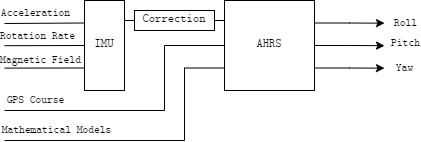
\includegraphics[height=1.3in]{background/ahrs.png}
\end{figure}

\subsection{Kalman Filter} \label{ssec:kalman_filter}
The Kalman Filter is a recursive algorithm introduced in the 1960's as a method to track, estimate, and predict the state of a system and corresponding uncertainties [CITE].
This filter integrates a dynamic (linear) model of the system, control inputs, measurements, and biases/uncertainties into a single algorithm.
This effectively fuses together system inputs and responses and extrapolates what the system is currently doing and expected to do.
One key advantage of this algorithm is that it only requires the guess of the previous state to estimate the current state. 
This massively decreases the memory and processing costs as the history of inputs, measurements, and uncertainties does not need to be remembered or analyzed.
However, it does have some limitations when the sensor data is noisy or the control inputs cannot be linearly mapped to the system state.
Random errors in the sensor data may cause the filter to behave unpredictably and non-linearity prevents proper fusion entirely.

The algorithm works by taking uncertainties from sensor measurements and using those to determine the Kalman Gain factor, $K_n$.
This gain is the magnitude of the uncertainties from the previous estimate and measurement sources.

\begin{equation} \label{eq:kalman_gain}
    \begin{aligned}
        K_n &= \frac{\text{Estimate Uncertainty}}{\text{Estimate Uncertainty + Measurement Uncertainty}} \\
            &= \frac{p_{n,n-1}}{p_{n,n-1} + r_n}
    \end{aligned}
\end{equation}

The gain is then applied to a state update equation where the current estimate of the sensor values is determined.

\begin{equation} \label{eq:kalman_state_update_eq}
    \begin{aligned}
        \hat{x}_{n,n} &= \hat{x}_{n,n-1} + K_n(z_n - \hat{x}_{n,n-1}) \\
                      &= (1-K_n)\hat{x}_{n,n-1} + K_n z_n \\
    \end{aligned}
\end{equation}

On the first run of the algorithm, an initial state guess and uncertainty are introduced as a starting point for the state prediction equation.
This equation is the mathematical model of the system and, for example, can be the Newtonian equations of motion for a moving body.
This creates a prediction for the next state.
The algorithm can then output the current state, predicted next state, and associated uncertainties with reasonably high accuracy - assuming the filter is tuned.
Tuning the filter can be done by better quantifying the measurement errors and by tuning hyperparameter called "process noise variables".
These variables control how much the algorithm depends on the measurement or the previous estimate to make the current and future estimates.

\begin{figure}[h!]
    \caption[Kalman filter block diagram]{Basic block diagram of a Kalman filter.}
    \label{fig:kalman_filter}
    \centering
    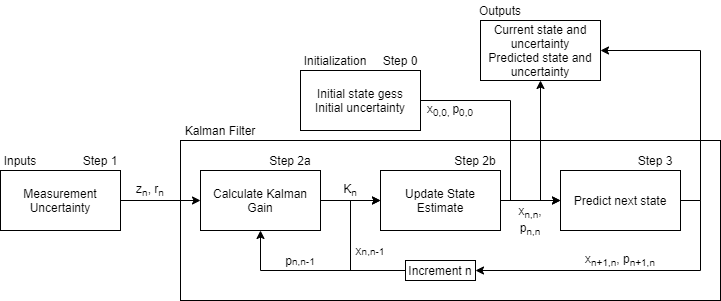
\includegraphics[width=6in]{background/KalmanFilter.png}
\end{figure}

\subsection{Mahony Filter} \label{ssec:bkg_mahony_filter}
A popular AHRS sensor fusion algorithm is the Mahony filter [CITE].
This algorithm estimates the rotation rate, $\pmb{\omega}'$ of the body given the instantaneous rotation rate, $\pmb{\omega}$ and acceleration vector, \pmb{a}.
The error, $e$, is calculated as the cross-product between the current acceleration vector and the expected gravitational acceleration vector from the previous estimate.
The filter uses a Proportional-Integral (PI) controller to determine the filter error from the previous estimate and apply a bias, $\delta\omega$ to the current estimate.
By integrating $\omega'$, the estimated attitude can be determined.
The equation for a basic Mahony figure is given below:

\begin{gather}
    \label{eq:mahony_filter}
    \pmb{\omega}' = \pmb{\omega} + \left(K_p + K_i\frac{1}{s}\right) \pmb{a} \times \pmb{d} \\
    \begin{aligned}
        \text{where } & \pmb{\omega} \text{ is the instantaneous rotation rate vector} \\
        & K_p \text{ is the proportional controller constant} \\
        & K_i \text{ is the integral controller constant} \\
        & \pmb{a} \text{ is the instantaneous acceleration vector} \\
        & \pmb{d} \text{ is the estimated gravity vector from the previous estimate} \\
    \end{aligned} \notag
\end{gather}

This filter is used to fuse 6DOF IMU data, but is limited as the yaw orientation cannot be known or calculated; it also does not account for gyroscopic drift which decreases its accuracy over time.
Additionally, this filter primarily works in the Eulerian coordinate system, which causes singularities and discontinuities due to gimbal lock.

\subsection{Madgwick Filter} \label{ssec:bkg_madgewick_filter}
To address the issues of the Mahony filter, Madgewick [CITE] proposed a different orientation filter, based on Mahony's work, that used quaternions throughout the calculations and could integrate magnetometer data for yaw estimation.
The use of quaternions throughout the entire filter eliminates the Eulerian singularities and improves performance.
Additionally, Madgewick's implementation considers the estimation bias to be an optimization problem solved by gradient-descent.
The gradient-descent approach allows the algorithm to have a much higher performance at lower sample rates and incorporate online magnetic distortion and gyroscopic drift compensation.

The filter uses accelerometer and magnetometer measurements to estimate the body's tilt and yaw relative to the geodetic frame of reference.
This gives an estimate of the direction vector for the error vector.
The magnitude of the error is determined via gradient-descent and subtracted from the gyroscope readings along the direction vector.
This computes an accurate rate of change vector, $\pmb{\dot{q}_t}$, that can be numerically integrated to yield the estimated orientation vector, $\pmb{q_t}$.

\subsection{Fast Complimentary Filter}


\section{Orientation and Rotation} \label{ssec:bkg_orientation}
A body can be rotated in 3D space along the x-, y-, and z-axis.
\textbf{Roll ($\phi$)} defines rotation about the x-axis; \textbf{pitch ($\theta$)} defines rotation about the y-axis; and \textbf{yaw ($\psi$)} defines rotation about the z-axis.
These three rotations are known as Euler angles.
They are easy to conceptually understand and model, but they are not mathematically pure.

\begin{figure}[h!]
    \caption[Body rotations]{Basic look at a 3D body and the axes of rotation in the body reference frame.}
    \label{fig:body_rotations}
    \centering
    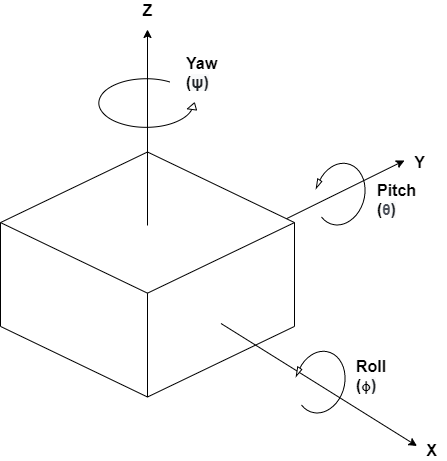
\includegraphics[height=2.5in]{background/body_rotations.png}
\end{figure}

A body can be rotated around all three axes to change its orientation and represented as the vector, $\langle\phi, \theta, \psi\rangle$.
The rotation can occur in a certain sequence, e.g. roll 45 degrees, pitch 45 degrees, then yaw 45 degrees.
This is simple to do so long as two of the rotation axes are not parallel to each other.
When two axes are parallel, they lock together in a condition called, "gimbal lock". 
We can overcome gimbal lock by adding a fourth dimension that can drive each axis independently.
This moves the rotation from the typical three dimensional space to the four dimensional, Hamiltonian, space.
We can represent this orientation as a four dimensional vector called a "quaternion".
This vector is more prevalent in modern AHRS design as it is more mathematically pure and means you do not have to determine if you need to change a rotation sequence to avoid or get out of gimbal lock.

It is possible to freely switch between Euler and quaternion vectors using trigonometric operations inside of a matrix multiplication operation.

\begin{figure}
    \begin{fitbox}[frametitle=Aside: Gimbal Lock]
        When two axes become parallel, eulerian changes to either axis become irrelevant, ergo, the system loses a degree of freedom.
        When in gimbal lock, rotations and plotting yield discontinuities that need to be mitigated by changing the rotation order, or moving two or three axes at once.
        This can create strange pathways for the body and cause unexpected behavior.
        
        The figure below shows a body's rotation while in gimbal lock. The rotation order is roll, pitch, then yaw.
        First, it is pitched 90 degrees upwards to align the roll and yaw axes, $\langle0, 90, 0\rangle$.
        If we then want to rotate it such that it's orientation is $\langle90, 0, 0\rangle$, it would be rolled left 90 degrees and pitched down 90 degrees.
        However, due to gimbal lock, the body ended up in the orientation $\langle0, 0, 90\rangle$!
        To break the gimbal lock and get to the correct orientation, the rotation order would have to be changed to pitch, yaw, roll, or the roll and yaw axes driven simultaneously.
        \begin{center}
            \subfloat[Start: $\langle0, 0, 0\rangle$]{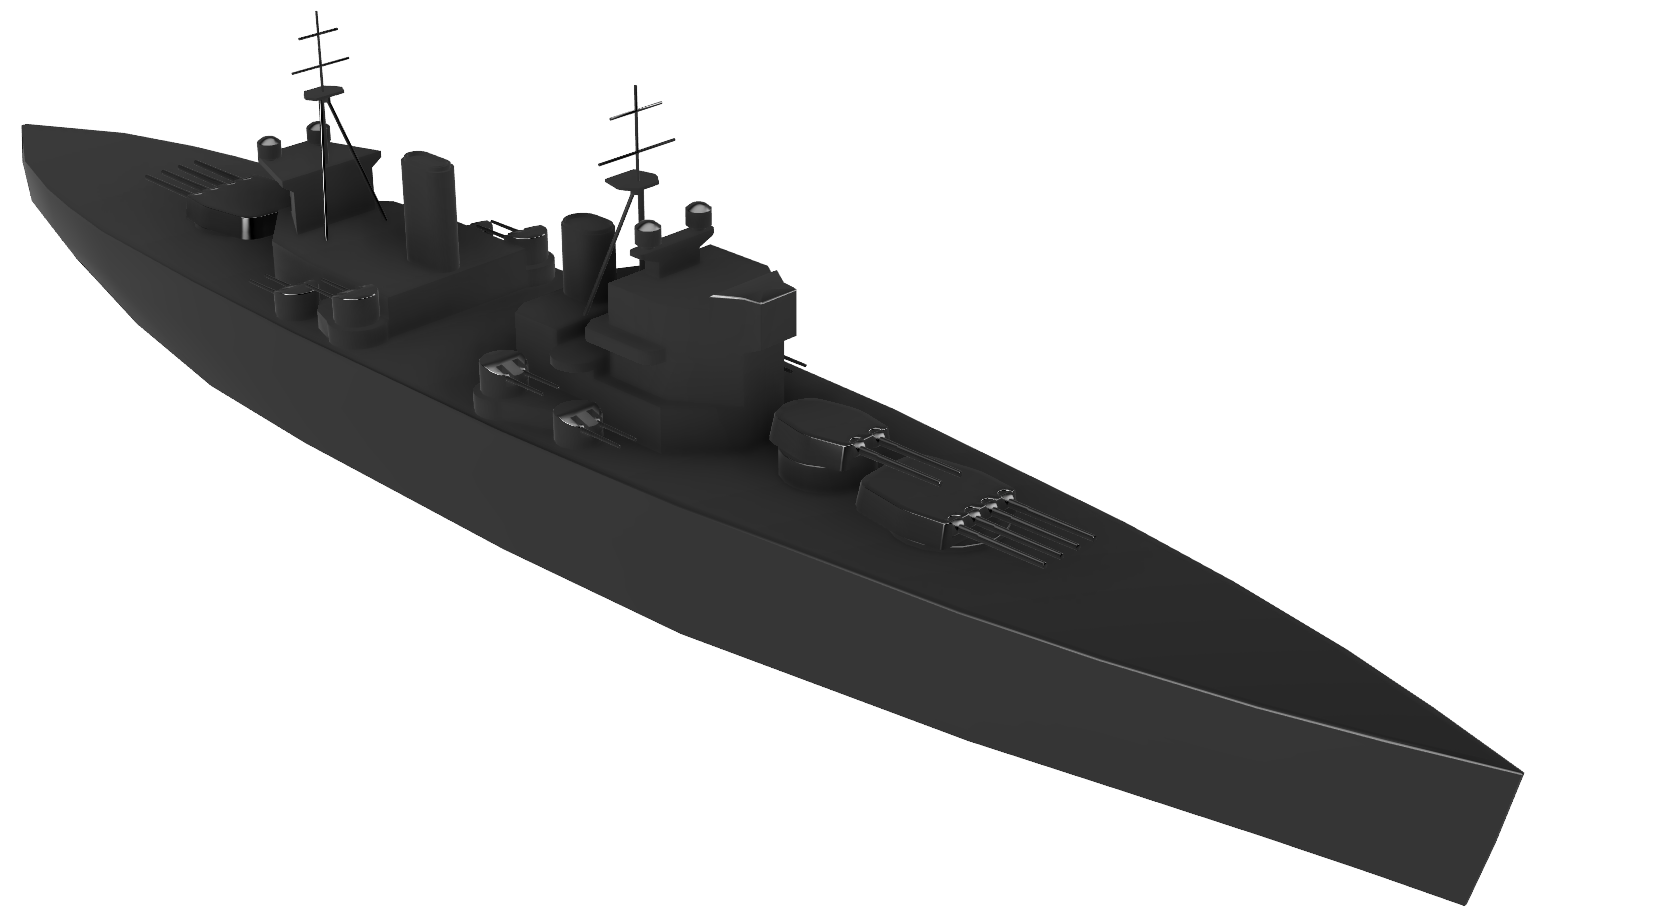
\includegraphics[width=0.25\textwidth]{background/ship_000000}\label{subfig:ship_000000}}\hskip3ex
            \subfloat[$\langle0, 90, 0\rangle$]{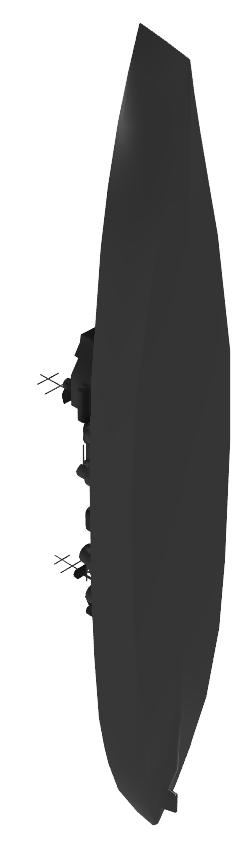
\includegraphics[height=1in]{background/ship_009000}\label{subfig:ship_009000}}\hskip10ex
            \subfloat[$\langle90, 90, 0\rangle$]{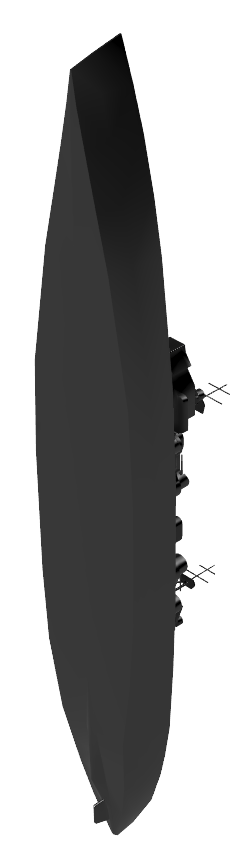
\includegraphics[height=1in]{background/ship_909000}\label{subfig:ship_909000}}\hskip5ex
            \subfloat[End: $\langle0, 0, 90\rangle$]{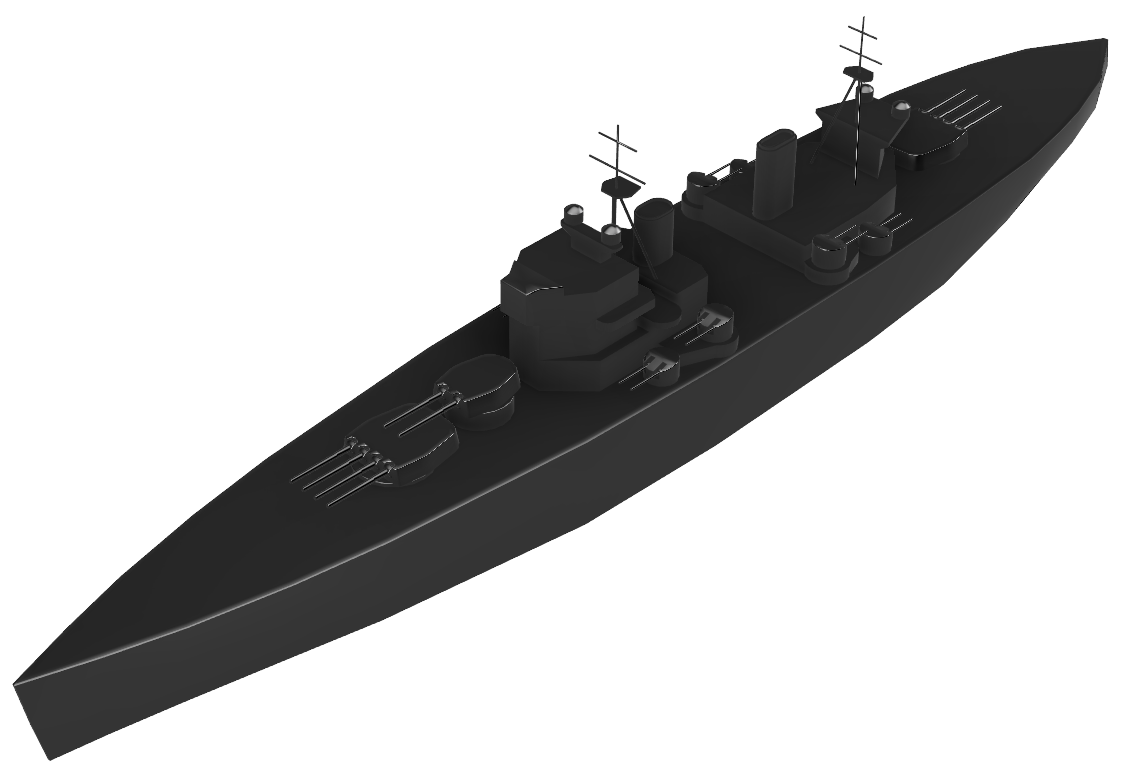
\includegraphics[width=0.25\textwidth]{background/ship_000090}\label{subfig:ship_000090}}
            \caption[Gimbal lock demonstration]{Demonstration of gimbal lock on a rotating 3D body.
            Despite only pitching and rolling the body, the end result of the transformation is an effective yaw.
            This is because the first pitch aligns the roll and yaw axes, effectively making them the same.
            In the given rotation order, any roll rotation would be equivalent to a yaw rotation when the object is pitched 90$^{\circ}$.
            \textit{3D model courtesy of "printable models" from Free3D.com.}}
        \end{center}
    \end{fitbox}
\end{figure}